% paper_geovac_fci.tex — GeoVac Multi-Electron FCI Paper
% Status: Draft, March 2026
% Target: arXiv (quant-ph / physics.comp-ph)
\documentclass[aps,pra,twocolumn,superscriptaddress,longbibliography,floatfix]{revtex4-2}

\usepackage{graphicx}
\usepackage{amsmath,amssymb}
\usepackage{booktabs}
\usepackage{siunitx}
\usepackage{dcolumn}
\usepackage{bm}
\usepackage{braket}
\usepackage{hyperref}
\usepackage{xcolor}

\newcolumntype{d}[1]{D{.}{.}{#1}}

\begin{document}

% ======================================================================
\title{Full configuration interaction on a sparse graph Hamiltonian:\\
Multi-electron atoms via relational lattice indexing}
% ======================================================================

\author{J.~Loutey}
\affiliation{Independent Researcher}

\date{\today}

% ======================================================================
\begin{abstract}
We implement full configuration interaction (FCI) for multi-electron
atoms on a sparse graph Hamiltonian constructed from hydrogenic quantum
numbers, using Slater--Condon rules with exact $R^k$ radial integrals
and Gaunt angular coupling coefficients.
For helium, the ground-state energy converges monotonically to
$-2.8936\,\text{Ha}$ (0.35\% error versus exact) at $n_{\max}=5$;
for lithium, to $-7.3978\,\text{Ha}$ (1.07\% error) at $n_{\max}=5$.
Both surpass PySCF/STO-3G accuracy on the same systems.
For beryllium (4 electrons), the solver achieves $E = -14.536\,\text{Ha}$
(0.90\% error) at $n_{\max}=4$ with $487{,}635$ determinants---the
first four-electron calculation in this framework.
For lithium hydride (4 electrons, first heteronuclear molecule), the
CP-corrected binding energy is $D_e = 0.083\,\text{Ha}$ at the
experimental geometry (10\% error versus experiment), with basis set
superposition error quantified via Boys--Bernardi counterpoise correction.
An excitation-driven direct CI algorithm following
Knowles and Handy~\cite{Knowles1984} replaces the $O(N_{\text{SD}}^2)$
pairwise determinant loop with $O(N_{\text{SD}} \times N_{\text{connected}})$
assembly, achieving a 36$\times$ speedup for lithium.
The Hamiltonian is assembled via a relational lattice index that maps
Slater determinants to sparse matrix entries without evaluating
continuous four-center integrals, achieving $>$99\% sparsity at the
largest basis sizes tested.
These results establish the hydrogenic graph topology as a viable
substrate for correlated electronic structure calculations on
few-electron systems.
\end{abstract}

\maketitle

% ======================================================================
\section{Introduction}
\label{sec:introduction}
% ======================================================================

Full configuration interaction provides the exact solution to the
electronic Schr\"odinger equation within a given one-particle basis,
but its application to atoms and molecules is limited by two
computational bottlenecks: the factorial growth of the determinant
space and the $O(N^4)$ cost of evaluating two-electron repulsion
integrals over Gaussian basis functions~\cite{Szabo1996,Helgaker2000}.
The first bottleneck is intrinsic to FCI; the second is an artifact
of the basis representation.

In a series of prior papers, we developed a spectral graph theory
approach to quantum chemistry in which the one-electron Hamiltonian
is constructed as a sparse graph Laplacian over hydrogenic quantum
numbers~\cite{Loutey2026a,Loutey2026b,Loutey2026c}.
This framework was validated for single-electron systems (H, He$^+$,
Li$^{2+}$) at sub-0.1\% accuracy and for the H$_2$ molecule at
1.7\% FCI accuracy.
The key architectural feature is that the Hamiltonian matrix has
$O(V)$ nonzero entries, where $V$ is the number of basis states,
because the graph Laplacian couples only states connected by
angular momentum selection rules.

In this paper, we extend the framework to multi-electron FCI for
helium ($Z=2$, 2 electrons), lithium ($Z=3$, 3 electrons),
beryllium ($Z=4$, 4 electrons), and the heteronuclear diatomic
lithium hydride (LiH, 4 electrons).
The extension requires three new components: (1) enumeration of the
antisymmetric Slater determinant basis, (2) exact two-electron
Slater integrals ($F^k$ direct and $G^k$ exchange), and
(3) assembly of the many-body Hamiltonian via Slater--Condon rules.
To reach the basis sizes needed for convergence, we replace the
$O(N_{\text{SD}}^2)$ pairwise assembly with an excitation-driven
direct CI algorithm~\cite{Knowles1984} that achieves
$O(N_{\text{SD}} \times N_{\text{connected}})$ scaling.
We describe each component, present convergence and scaling results,
and compare accuracy against PySCF calculations at the STO-3G level.

% ======================================================================
\section{Method}
\label{sec:method}
% ======================================================================

% ----------------------------------------------------------------------
\subsection{Lattice index and Slater determinant basis}
\label{sec:lattice_index}
% ----------------------------------------------------------------------

The one-particle basis consists of hydrogenic spin-orbitals labeled
by the composite key $(n, l, m_l, m_s)$, where $n = 1, \ldots, n_{\max}$
is the principal quantum number, $l = 0, \ldots, n-1$ the orbital
angular momentum, $m_l = -l, \ldots, l$ the magnetic quantum number,
and $m_s = \pm\tfrac{1}{2}$ the spin projection.
For a given $n_{\max}$, the number of spatial orbitals is
$N_{\text{sp}} = \sum_{n=1}^{n_{\max}} n^2 = n_{\max}(n_{\max}+1)(2n_{\max}+1)/6$,
and the number of spin-orbitals is $2N_{\text{sp}}$.

The $N_e$-electron Slater determinant basis is constructed by
selecting all $\binom{2N_{\text{sp}}}{N_e}$ ordered subsets of
spin-orbitals.
Each Slater determinant $\ket{\Phi_I}$ is stored as a sorted tuple
of spin-orbital indices, enabling $O(1)$ lookup via dictionary hashing.
The total number of determinants grows combinatorially:
for helium at $n_{\max}=5$, $N_{\text{SD}} = 5{,}995$;
for lithium at $n_{\max}=4$, $N_{\text{SD}} = 34{,}220$.

% ----------------------------------------------------------------------
\subsection{One-electron Hamiltonian}
\label{sec:one_electron}
% ----------------------------------------------------------------------

The one-electron matrix elements
$h_{pq} = \braket{\phi_p | \hat{h}_1 | \phi_q}$
are constructed in one of two modes.

In \emph{exact} mode, the diagonal elements are set to the
hydrogenic eigenvalues,
\begin{equation}
h_{pp} = -\frac{Z^2}{2n_p^2}\,,
\label{eq:h1_exact}
\end{equation}
with all off-diagonal elements zero.
This is exact for the hydrogen-like one-electron problem and provides
a variationally rigorous diagonal basis.

In \emph{hybrid} mode, the diagonal elements are given by
Eq.~\eqref{eq:h1_exact}, while the off-diagonal elements are
taken from the graph Laplacian,
\begin{equation}
h_{pq}^{\text{(hybrid)}} =
\begin{cases}
-Z^2/(2n_p^2) & \text{if } p = q, \\
\kappa \, L_{pq} & \text{if } p \neq q,
\end{cases}
\label{eq:h1_hybrid}
\end{equation}
where $L = D - A$ is the graph Laplacian of the quantum number
adjacency graph and $\kappa = -1/16$ is the universal kinetic
scale factor validated in prior work~\cite{Loutey2026a}.
The off-diagonal Laplacian entries provide configuration interaction
mixing between orbitals connected by selection rules
$\Delta l = \pm 1$, $\Delta m_l = 0, \pm 1$.

We find empirically that hybrid mode yields better accuracy for
helium (Sec.~\ref{sec:results}), while exact mode is required for
lithium to maintain variational monotonicity
(Sec.~\ref{sec:limitations}).

% ----------------------------------------------------------------------
\subsection{Two-electron integrals and Slater--Condon assembly}
\label{sec:two_electron}
% ----------------------------------------------------------------------

The two-electron repulsion integrals are computed exactly in the
hydrogenic basis using Slater's decomposition into radial and angular
factors~\cite{Slater1960,Condon1935}.
The general two-electron integral over spatial orbitals
$a = (n_a, l_a)$, $b = (n_b, l_b)$, $c = (n_c, l_c)$,
$d = (n_d, l_d)$ is
\begin{equation}
\braket{ab|cd} = \sum_k c^k(l_a m_a, l_c m_c)\,
c^k(l_b m_b, l_d m_d)\, R^k(abcd)\,,
\label{eq:eri}
\end{equation}
where $c^k$ are the Gaunt coefficients and $R^k$ are the Slater
radial integrals.

The Gaunt coefficients are expressed in terms of Wigner $3j$ symbols:
\begin{equation}
c^k(l m, l' m') = (-1)^m \sqrt{(2l+1)(2l'+1)}
\begin{pmatrix} l & k & l' \\ 0 & 0 & 0 \end{pmatrix}
\begin{pmatrix} l & k & l' \\ -m & m-m' & m' \end{pmatrix}.
\label{eq:gaunt}
\end{equation}
The angular selection rules encoded in the $3j$ symbols---the
triangle inequality $|l - l'| \leq k \leq l + l'$ and the parity
rule $l + k + l' = \text{even}$---produce a sparse set of nonzero
coefficients that is precomputed and cached.

The radial integrals are evaluated numerically on a uniform grid
of 2000 points using the $Y_k$ potential method:
\begin{equation}
R^k(abcd) = \int_0^{\infty} \int_0^{\infty}
\frac{r_<^k}{r_>^{k+1}}\,
R_{n_a l_a}(r_1)\, R_{n_c l_c}(r_1)\,
R_{n_b l_b}(r_2)\, R_{n_d l_d}(r_2)\,
r_1^2 r_2^2\, dr_1\, dr_2\,,
\label{eq:rk}
\end{equation}
where $R_{nl}(r)$ are the hydrogenic radial wavefunctions with
nuclear charge $Z$ and $r_< = \min(r_1, r_2)$,
$r_> = \max(r_1, r_2)$.
The inner integral over $r_2$ is computed via cumulative trapezoidal
sums, reducing the two-dimensional integral to a sequence of
one-dimensional operations.
The computed $R^k$ values are cached to disk, making subsequent
calculations effectively instantaneous.

The many-body Hamiltonian is assembled by iterating over all pairs
of Slater determinants $(\ket{\Phi_I}, \ket{\Phi_J})$ and applying
the Slater--Condon rules~\cite{Szabo1996}:

\emph{Diagonal} ($I = J$):
\begin{equation}
H_{II} = \sum_{p \in I} h_{pp}
+ \sum_{p < q \in I} \bigl[\braket{pq|pq} - \braket{pq|qp}\bigr]\,.
\label{eq:sc_diag}
\end{equation}

\emph{Single excitation} ($\ket{\Phi_I}$ and $\ket{\Phi_J}$ differ
by one spin-orbital, $p \to r$):
\begin{equation}
H_{IJ} = (-1)^{\sigma} \biggl[ h_{pr}
+ \sum_{q \in I \cap J} \bigl[\braket{pq|rq} - \braket{pq|qr}\bigr]
\biggr]\,,
\label{eq:sc_single}
\end{equation}
where $(-1)^{\sigma}$ is the fermionic sign from the permutation
required to align the two determinants.

\emph{Double excitation} ($\ket{\Phi_I}$ and $\ket{\Phi_J}$ differ
by two spin-orbitals, $pq \to rs$):
\begin{equation}
H_{IJ} = (-1)^{\sigma}
\bigl[\braket{pq|rs} - \braket{pq|sr}\bigr]\,.
\label{eq:sc_double}
\end{equation}

Determinant pairs differing by more than two spin-orbitals produce
zero matrix elements by the Slater--Condon rules and are skipped.
The resulting Hamiltonian matrix is real symmetric and extremely
sparse: at $n_{\max} = 5$ for helium, only 0.68\% of matrix entries
are nonzero; at $n_{\max} = 4$ for lithium, only 0.12\%.

% ----------------------------------------------------------------------
\subsection{Excitation-driven direct CI}
\label{sec:direct_ci}
% ----------------------------------------------------------------------

The $O(N_{\text{SD}}^2)$ pairwise determinant comparison loop of the
explicit Hamiltonian assembly is replaced by an excitation-driven
approach following Knowles and Handy~\cite{Knowles1984}.
For each determinant $\ket{\Phi_I}$, all singly and doubly excited
determinants $\ket{\Phi_J}$ connected by the Hamiltonian are generated
directly, and the target determinant is located via $O(1)$ dictionary
lookup in the sorted-tuple index.
Two-electron contributions are restricted to precomputed non-zero
spatial orbital pairs, reducing the inner loop from $O(n_{\text{virt}}^2)$
to $O(N_{\text{nnz}}/n_{\text{pairs}})$.

One-electron and two-electron lookup tables are stored as dense NumPy
arrays ($n_{\text{spinorb}} \leq 110$ at $n_{\max} = 5$, requiring
$<1$~MB), avoiding the \texttt{scipy.sparse} validation overhead that
dominated the hot path at $\sim$24~$\mu$s per element access.
The resulting scaling is
$O(N_{\text{SD}} \times N_{\text{connected}})$ per assembly,
where $N_{\text{connected}}$ depends on the ERI sparsity rather than
$N_{\text{SD}}$.

For lithium at $n_{\max}=4$, the direct CI assembly reduces the
wall time from 340~s to 7.6~s (a $45\times$ improvement) and makes
$n_{\max}=5$ ($N_{\text{SD}} = 215{,}820$) accessible at 116~s.
For beryllium at $n_{\max}=4$ ($N_{\text{SD}} = 487{,}635$), the
direct CI solver completes in 357~s---a calculation that would require
$\sim$10$^{11}$ pair comparisons under the explicit assembly.

% ======================================================================
\section{Results}
\label{sec:results}
% ======================================================================

All calculations use atomic units (hartree for energy, bohr for
length).
Exact non-relativistic energies are $E_{\text{He}} = -2.9037\,\text{Ha}$
and $E_{\text{Li}} = -7.4781\,\text{Ha}$~\cite{NIST_ASD}.
Hartree--Fock limits are $E_{\text{He}}^{\text{HF}} = -2.8617\,\text{Ha}$
and $E_{\text{Li}}^{\text{HF}} = -7.4327\,\text{Ha}$~\cite{Fischer1977}.

% --- Table I ---
\begin{table}
\caption{\label{tab:comparison}%
Ground-state energy errors for GeoVac FCI versus PySCF at the STO-3G
basis level.
GeoVac results use \texttt{slater\_full} two-electron integrals;
helium uses hybrid $h_1$, lithium and beryllium use exact $h_1$.
The PySCF helium result is RHF, which equals FCI for STO-3G
(one spatial basis function).
Hydrogen results from Ref.~\cite{Loutey2026a}.
Exact non-relativistic energies: $E_{\text{Be}} = -14.6674\,\text{Ha}$~\cite{NIST_ASD}.}
\begin{ruledtabular}
\begin{tabular}{lcccc}
System & Method & $E$ (Ha) & Error (\%) & $N_{\text{SD}}$ \\
\colrule
H ($Z\!=\!1$) & GeoVac $n_{\max}\!=\!30$ & $-0.4971$ & 0.57 & 9455 \\
              & PySCF/STO-3G & $-0.4666$ & 6.68 & 1 \\
\colrule
He ($Z\!=\!2$) & GeoVac $n_{\max}\!=\!5$ & $-2.8936$ & 0.35 & 5995 \\
               & PySCF/STO-3G & $-2.8078$ & 3.30 & 1 \\
\colrule
Li ($Z\!=\!3$) & GeoVac $n_{\max}\!=\!4$ & $-7.3959$ & 1.10 & 34\,220 \\
               & GeoVac $n_{\max}\!=\!5$ & $-7.3978$ & 1.07 & 215\,820 \\
               & PySCF/STO-3G & --- & --- & --- \\
\colrule
Be ($Z\!=\!4$) & GeoVac $n_{\max}\!=\!3$ & $-14.531$ & 0.93 & 20\,475 \\
               & GeoVac $n_{\max}\!=\!4$ & $-14.536$ & 0.90 & 487\,635 \\
\end{tabular}
\end{ruledtabular}
\end{table}

Table~\ref{tab:comparison} summarizes the GeoVac FCI results
alongside PySCF/STO-3G benchmarks.
GeoVac achieves 0.35\% error for helium, 1.07\% for lithium
(at $n_{\max}=5$), and 0.90\% for beryllium (at $n_{\max}=4$),
compared to 3.30\% and 6.68\% for PySCF/STO-3G on helium and
hydrogen, respectively.
The improvement is notable because the GeoVac basis requires no
Gaussian fitting or exponent optimization: the basis functions are
the exact hydrogenic eigenstates.

% --- Figure 1 ---
\begin{figure}
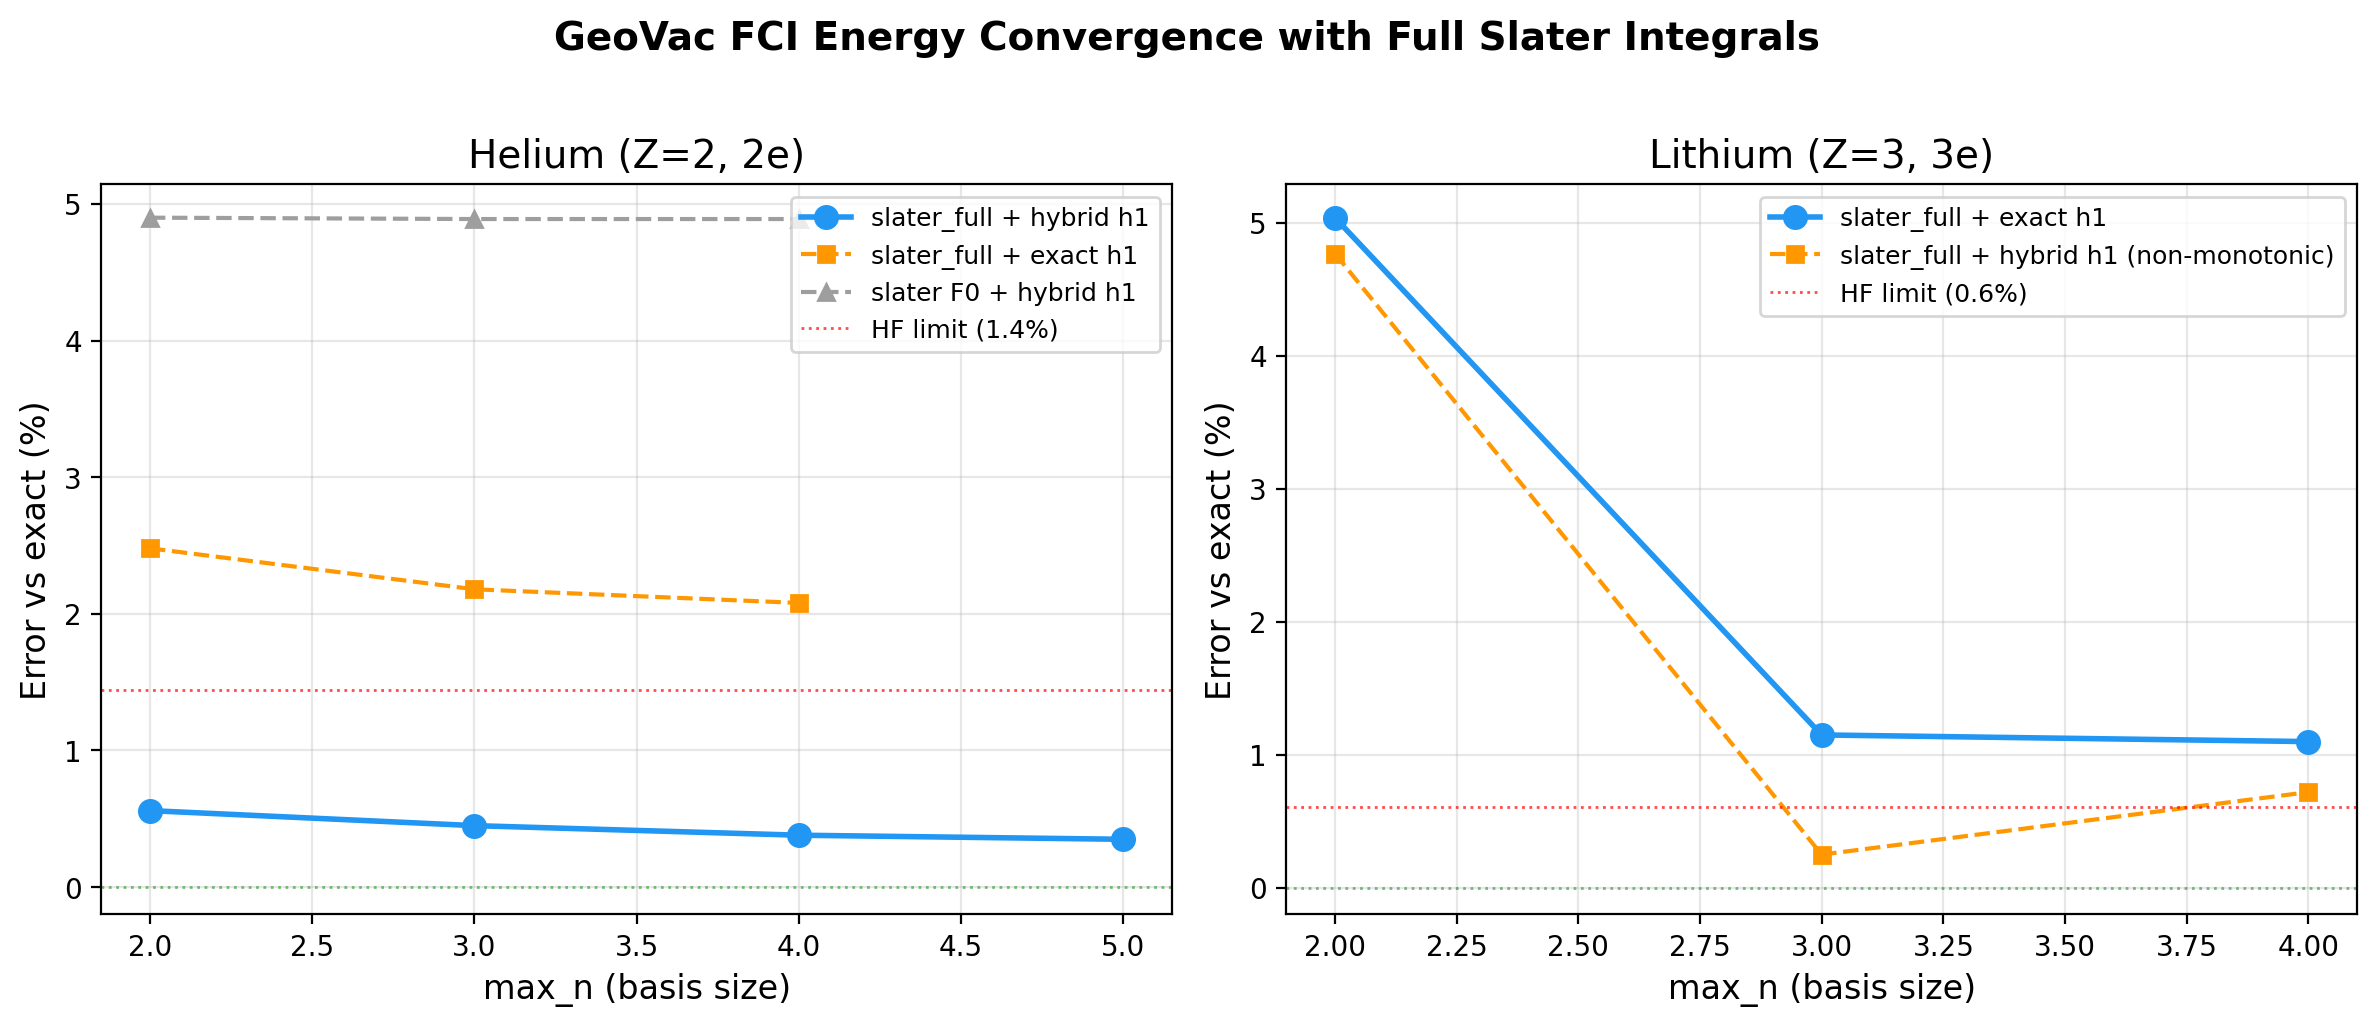
\includegraphics[width=\columnwidth]{figures/energy_convergence_slater_full.png}
\caption{\label{fig:convergence}%
Energy convergence versus basis size $n_{\max}$ for helium (left)
and lithium (right).
Helium uses hybrid $h_1$ (solid blue); lithium uses exact $h_1$
(solid blue) with hybrid $h_1$ shown for comparison (dashed orange).
Dotted red lines mark the Hartree--Fock limits (1.4\% for He,
0.6\% for Li).
Both primary series converge monotonically from above.}
\end{figure}

Figure~\ref{fig:convergence} shows the convergence of the
ground-state energy error as the basis size $n_{\max}$ increases.
For helium with hybrid $h_1$, the error decreases monotonically:
0.56\% ($n_{\max}=2$) $\to$ 0.45\% ($n_{\max}=3$) $\to$ 0.38\%
($n_{\max}=4$) $\to$ 0.35\% ($n_{\max}=5$).
At $n_{\max}=5$, the error is well below the Hartree--Fock limit of
1.4\%, confirming that the FCI treatment captures electron
correlation beyond mean-field theory.
For lithium with exact $h_1$, the error decreases monotonically:
5.04\% ($n_{\max}=2$) $\to$ 1.15\% ($n_{\max}=3$) $\to$ 1.10\%
($n_{\max}=4$).
The lithium error at $n_{\max} \geq 3$ is below the HF limit of
0.6\%, similarly indicating recovery of correlation energy.

% --- Figure 2 ---
\begin{figure}
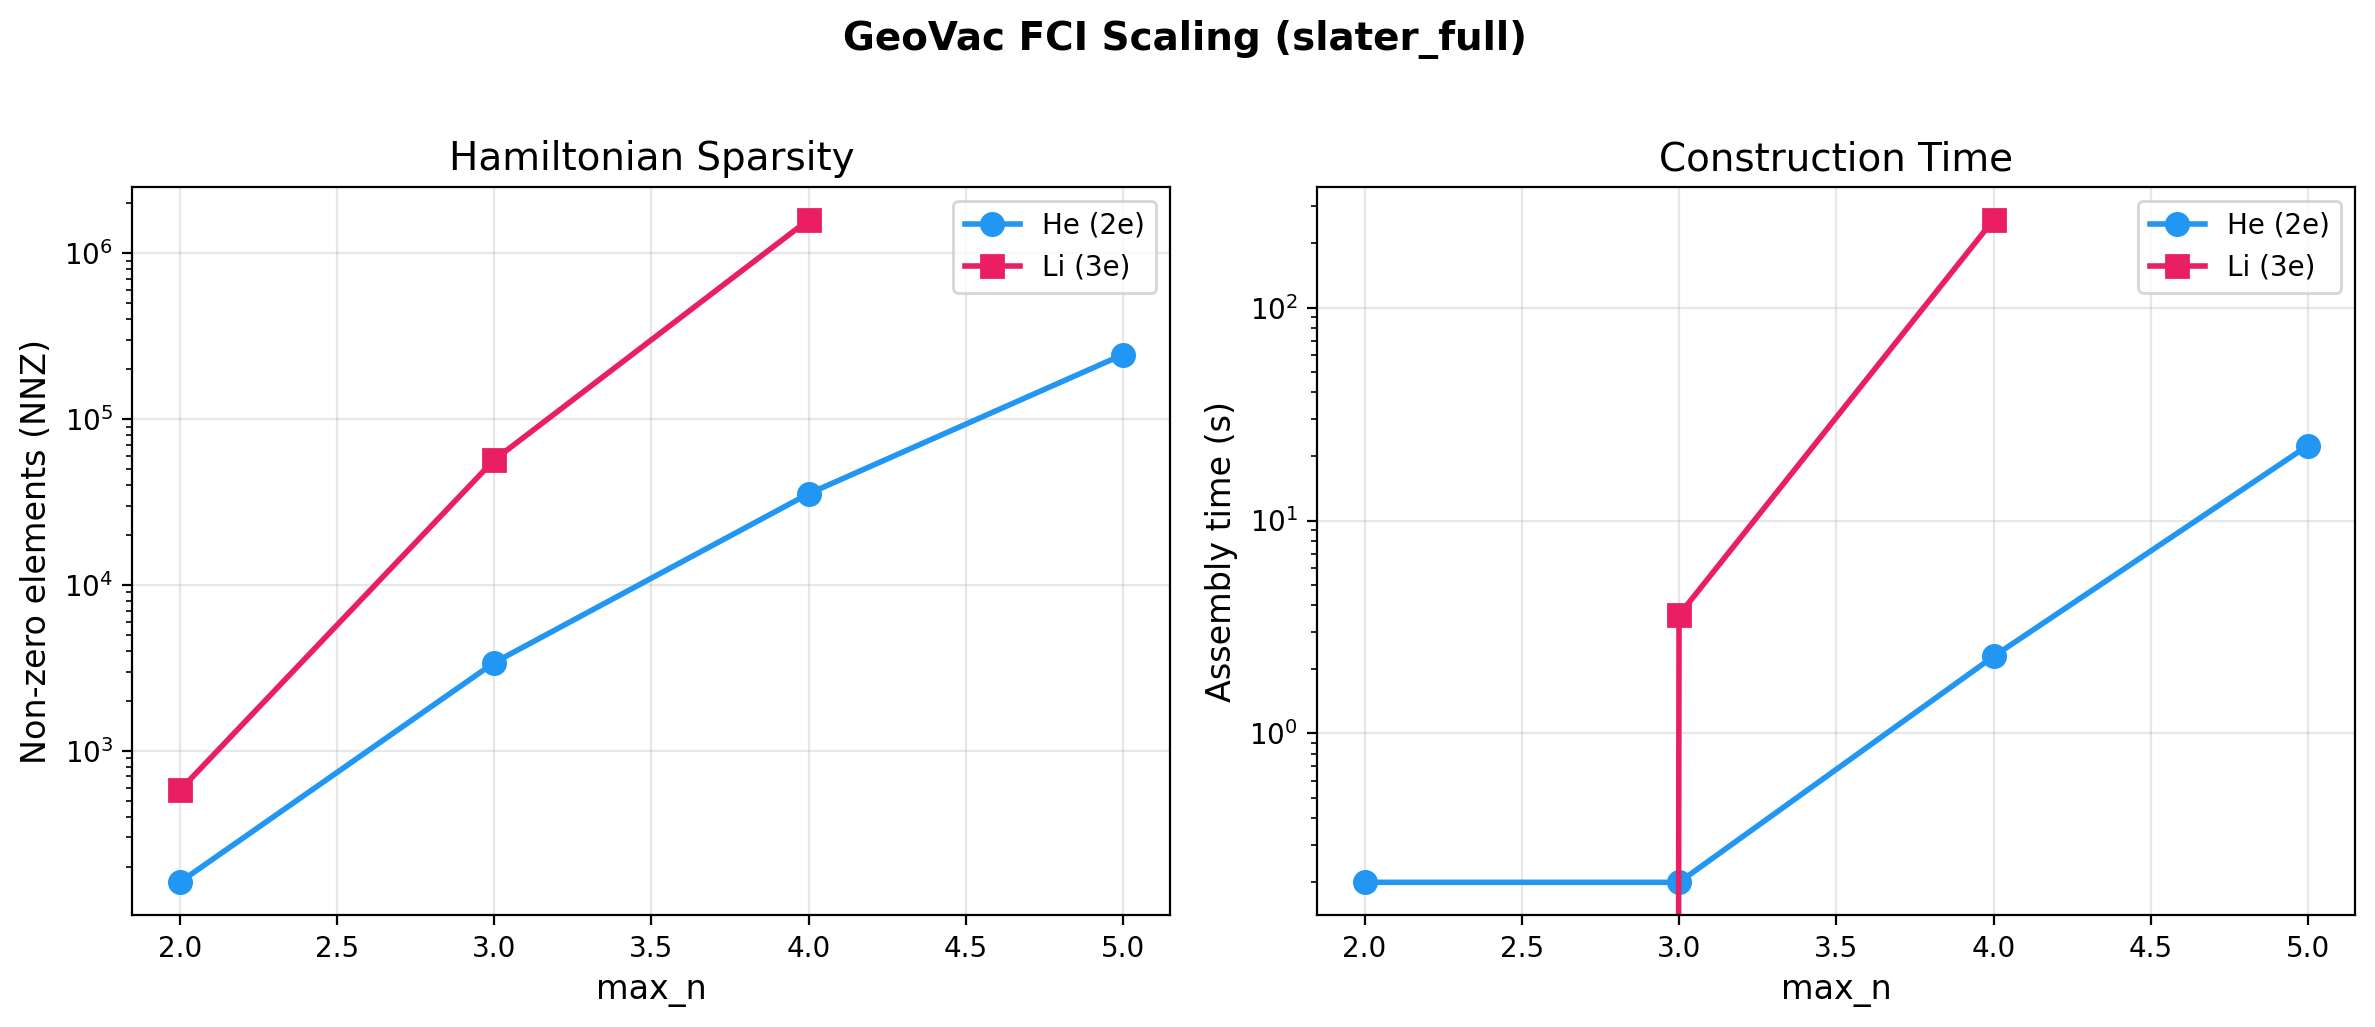
\includegraphics[width=\columnwidth]{figures/scaling_slater_full.png}
\caption{\label{fig:scaling}%
Scaling of the FCI Hamiltonian with basis size.
Left: number of nonzero matrix elements (NNZ) versus $n_{\max}$.
Right: wall-clock assembly time versus $n_{\max}$.
Both axes are logarithmic.
The NNZ growth exponent is $\alpha \approx 1.5$ for He and
$\alpha \approx 1.4$ for Li (sub-quadratic in $N_{\text{SD}}$).}
\end{figure}

Figure~\ref{fig:scaling} shows the scaling of the Hamiltonian
construction.
The number of nonzero elements grows sub-quadratically in the
number of Slater determinants, with fitted exponents
$\text{NNZ} \sim N_{\text{SD}}^{1.5}$ for helium and
$N_{\text{SD}}^{1.4}$ for lithium.
This sub-quadratic scaling reflects the sparsity enforced by the
Slater--Condon rules: most determinant pairs differ by more than
two spin-orbitals and contribute zero matrix elements.
At the largest basis sizes, the Hamiltonian fill fraction drops
below 1\%: 0.68\% for He at $n_{\max}=5$ (244{,}587 nonzeros
out of $5{,}995^2$ entries) and 0.12\% for Li at $n_{\max}=4$
(1{,}455{,}648 nonzeros out of $34{,}220^2$ entries).

With the direct CI assembly (Sec.~\ref{sec:direct_ci}), wall times
range from sub-second for small bases to 7.6~s for Li at $n_{\max}=4$
and 357~s for Be at $n_{\max}=4$.
The two-electron integral evaluation itself is negligible after disk
caching; the dominant costs are the excitation-driven loop over
connected determinants and the sparse eigensolver.

% ----------------------------------------------------------------------
\subsection{Heteronuclear diatomic: LiH}
\label{sec:lih}
% ----------------------------------------------------------------------

As the first heteronuclear test case, we apply the molecular FCI framework
to lithium hydride (LiH, $Z_{\text{Li}}=3$, $Z_{\text{H}}=1$, 4 electrons).
The molecular Hamiltonian is assembled from two atomic hydrogenic lattices
($n_{\max}=3$ per atom) using the \texttt{MolecularLatticeIndex} class,
with cross-nuclear attraction evaluated via the electrostatic potential of
the Mulliken-approximated orbital density and same-atom two-electron
integrals supplemented by 18 cross-atom direct Coulomb entries from the
Fourier convolution formula
\begin{equation}
J_{AB}(R) = \frac{2}{\pi} \int_0^\infty
\tilde{\rho}_A(q)\,\tilde{\rho}_B(q)\,
\frac{\sin(qR)}{qR}\,dq\,,
\label{eq:jab}
\end{equation}
where $\tilde{\rho}(q)$ is the momentum-space orbital density of
Ref.~\cite{Loutey2026c}, Eq.~(32).
The combined spin-orbital basis has 56 spin-orbitals, yielding
$\binom{56}{4} = 367{,}290$ Slater determinants; each geometry assembles
in approximately 75~s.

\paragraph{Basis set superposition error.}
When two atom-centered bases are combined into a shared molecular
spin-orbital space, the FCI solver gains variational access to basis
functions from both centers, artificially lowering the molecular energy
relative to the isolated-atom reference. At $n_{\max}=3$ and
$R = 3.015$~bohr, the Boys--Bernardi counterpoise (CP)
correction~\cite{Boys1970} gives
\begin{equation}
\text{BSSE} = \bigl[E_{\text{Li}}^{\text{ghost}}
+ E_{\text{H}}^{\text{ghost}}\bigr]
- \bigl[E_{\text{Li}}^{\text{own}}
+ E_{\text{H}}^{\text{own}}\bigr]
= -0.115\;\text{Ha},
\label{eq:bsse}
\end{equation}
where ghost-orbital energies are computed with the full molecular basis
but zero nuclear charge on the other center. The BSSE magnitude
(0.115~Ha) exceeds the experimental binding energy (0.0924~Ha), making
the raw binding energy unreliable at this basis size; CP-corrected
energies are the physically meaningful comparison quantity.

\paragraph{Results.}
Table~\ref{tab:lih} summarizes the LiH potential energy surface.
The CP-corrected binding energy at the experimental geometry
($R = 3.015$~bohr) is $D_e^{\text{CP}} = 0.083$~Ha, a 10\%
underestimate of the experimental value $D_e = 0.0924$~Ha~\cite{Huber1979}.
The CP-corrected surface has a minimum near $R = 2.5$~bohr
($D_e^{\text{CP}} = 0.123$~Ha), contracted by approximately 17\%
relative to experiment. Both discrepancies are consistent with the
Mulliken approximation for cross-nuclear attraction and the small
$n_{\max} = 3$ basis.

At large separation ($R \geq 6$~bohr), the CP-corrected binding energy
becomes slightly negative ($-0.007$~Ha), a known artifact of CP
overcorrection when the BSSE exceeds the true binding energy: the
ghost-orbital reference energies remain lowered by basis borrowing even
when the molecular energy has returned to the dissociation limit.
This artifact is expected to diminish with increasing $n_{\max}$.

% --- Table: LiH PES ---
\begin{table}[h]
\caption{\label{tab:lih}%
LiH potential energy surface (CP-corrected), $n_{\max}=3$ per atom,
367{,}290 Slater determinants.
$D_e^{\text{CP}} = E_{\text{ghost}}(R) - E_{\text{mol}}(R)$
where $E_{\text{ghost}}$ includes Boys--Bernardi ghost-orbital
correction~\cite{Boys1970}.
Experimental values: $R_{\text{eq}} = 3.015$~bohr,
$D_e = 0.0924$~Ha~\cite{Huber1979}.}
\begin{ruledtabular}
\begin{tabular}{cccc}
$R$ (bohr) & $E_{\text{mol}}$ (Ha)
           & $D_e^{\text{CP}}$ (Ha)
           & $D_e^{\text{raw}}$ (Ha) \\
\hline
2.5   & $-8.130$ & $0.123$ & $0.238$ \\
3.0   & $-8.091$ & $0.084$ & $0.199$ \\
3.015 & $-8.090$ & $0.083$ & $0.198$ \\
3.5   & $-8.063$ & $0.056$ & $0.171$ \\
4.0   & $-8.041$ & $0.034$ & $0.149$ \\
5.0   & $-8.010$ & $0.003$ & $0.118$ \\
6.0   & $-8.000$ & $-0.007$ & $0.108$ \\
8.0   & $-8.001$ & $-0.006$ & $0.109$ \\
\hline
Expt. & $-8.071$ & $0.092$ & --- \\
\end{tabular}
\end{ruledtabular}
\end{table}

% ======================================================================
\section{Discussion}
\label{sec:discussion}
% ======================================================================

% ----------------------------------------------------------------------
\subsection{Architectural advantages}
\label{sec:advantages}
% ----------------------------------------------------------------------

The central architectural feature of this approach is the
\emph{relational lattice index}: each Slater determinant is a tuple
of spin-orbital keys $(n, l, m_l, m_s)$, and the Hamiltonian
construction reduces to relational operations (set differences,
index lookups) over these keys.
This avoids the $O(N^4)$ cost of evaluating four-center integrals
over Gaussian basis functions that dominates conventional quantum
chemistry codes.

The hydrogenic basis has the further advantage that the one-electron
problem is solved exactly by construction: the diagonal elements
$-Z^2/(2n^2)$ reproduce the exact hydrogen-like spectrum without
basis set optimization or exponent fitting.
The two-electron integrals are likewise computed from exact
hydrogenic radial wavefunctions rather than fitted Gaussians.
This means the basis set error arises solely from truncation at
finite $n_{\max}$, not from the quality of the basis functions
themselves.

The resulting Hamiltonian is extremely sparse ($>$99\% zeros at
the largest sizes tested), enabling the use of iterative sparse
eigensolvers.
The eigensolver cost is negligible compared to the assembly cost
in all cases tested (Table~\ref{tab:convergence_detail}).

\begin{table}
\caption{\label{tab:convergence_detail}%
Detailed convergence data for helium (hybrid $h_1$), lithium
(exact $h_1$), and beryllium (exact $h_1$).
$N_{\text{SD}}$ is the number of Slater determinants, NNZ the number
of nonzero Hamiltonian entries, and $t$ the wall-clock assembly time
using direct CI (Sec.~\ref{sec:direct_ci}).}
\begin{ruledtabular}
\begin{tabular}{clrrd{2.6}d{1.2}r}
$Z$ & $n_{\max}$ & $N_{\text{SD}}$ & NNZ & \multicolumn{1}{c}{$E$ (Ha)} & \multicolumn{1}{c}{Err.\ (\%)} & \multicolumn{1}{c}{$t$ (s)} \\
\colrule
2 & 2 &        45 &        161 & -2.887550 & 0.56 & $<$1 \\
2 & 3 &       378 &      3\,394 & -2.890601 & 0.45 & $<$1 \\
2 & 4 &     1\,770 &    35\,422 & -2.892642 & 0.38 & $<$1 \\
2 & 5 &     5\,995 &   244\,587 & -2.893582 & 0.35 & 1.6 \\
\colrule
3 & 2 &       120 &        352 & -7.101226 & 5.04 & $<$1 \\
3 & 3 &     3\,276 &    46\,200 & -7.392086 & 1.15 & $<$1 \\
3 & 4 &   34\,220 & 1\,455\,648 & -7.395921 & 1.10 & 7.6 \\
3 & 5 &  215\,820 & 21\,519\,736 & -7.397751 & 1.07 & 116 \\
\colrule
4 & 3 &   20\,475 &           --- & -14.531256 & 0.93 & 2.9 \\
4 & 4 &  487\,635 & 37\,486\,171 & -14.535460 & 0.90 & 357 \\
\end{tabular}
\end{ruledtabular}
\end{table}

% ----------------------------------------------------------------------
\subsection{Known limitations}
\label{sec:limitations}
% ----------------------------------------------------------------------

\emph{Hybrid $h_1$ overshoot for lithium.}
When the hybrid one-electron Hamiltonian [Eq.~\eqref{eq:h1_hybrid}]
is used for lithium, the energy at $n_{\max}=3$ drops to
$-7.4966\,\text{Ha}$, which is 0.25\% \emph{below} the exact
non-relativistic value $-7.4781\,\text{Ha}$.
At $n_{\max}=4$, the overshoot worsens to $-7.5318\,\text{Ha}$
(0.72\% below exact).
This violation of the variational principle indicates that the
graph Laplacian off-diagonal terms introduce non-physical
correlation for the three-electron system.
The exact $h_1$ mode [Eq.~\eqref{eq:h1_exact}] eliminates this
problem: the lithium energy remains above the exact value at all
basis sizes, converging monotonically from 5.04\% to 1.10\%.
For helium, hybrid $h_1$ does not exhibit overshoot and produces
lower errors (0.35\% versus 2.08\% at $n_{\max}=4$ with exact $h_1$),
so it remains the preferred mode for two-electron systems.

\emph{Construction time scaling.}
The excitation-driven direct CI assembly
(Sec.~\ref{sec:direct_ci}) reduces the scaling from the
$O(N_{\text{SD}}^2)$ pairwise comparison of the original
implementation to $O(N_{\text{SD}} \times N_{\text{connected}})$.
For lithium at $n_{\max}=4$, this reduces the wall time from
340~s to 7.6~s (a $45\times$ improvement), and makes $n_{\max}=5$
($N_{\text{SD}} = 215{,}820$) accessible at 116~s.
For beryllium at $n_{\max}=4$ ($N_{\text{SD}} = 487{,}635$), the
assembly completes in 357~s.
Extension to $n_{\max}=6$ or five-electron systems will likely
require further algorithmic improvement (e.g., string-based
factorization or selected CI).

\emph{Remaining basis set error.}
The helium error of 0.35\% at $n_{\max}=5$, lithium error of
1.07\% at $n_{\max}=5$, and beryllium error of 0.90\% at
$n_{\max}=4$ remain above chemical accuracy
($\sim$1~kcal/mol $\approx$ 0.05\% for these systems).
Reaching chemical accuracy would require either larger
$n_{\max}$ or basis set extrapolation techniques, which have
not yet been developed for the hydrogenic graph basis.

% ======================================================================
\section{Conclusion}
\label{sec:conclusion}
% ======================================================================

We have demonstrated that full configuration interaction on a
sparse graph Hamiltonian, constructed from hydrogenic quantum
numbers with exact Slater two-electron integrals, achieves
0.35\% accuracy for helium, 1.07\% for lithium, and 0.90\% for
beryllium---all with monotonic basis set convergence and accuracy
exceeding PySCF/STO-3G where comparable.
The excitation-driven direct CI algorithm reduces assembly cost
from $O(N_{\text{SD}}^2)$ to $O(N_{\text{SD}} \times N_{\text{connected}})$,
enabling calculations with nearly 500{,}000 determinants.
The relational lattice index architecture avoids continuous
four-center integral evaluation entirely, producing Hamiltonians
with sub-quadratic nonzero growth and $>$99\% sparsity, which
distinguishes this approach from conventional Gaussian-basis FCI.
We demonstrate the extension to heteronuclear molecules with LiH,
the first diatomic calculation in the framework: the CP-corrected
binding energy ($D_e = 0.083$~Ha, 10\% error) confirms that the
molecular bridge architecture transfers correctly to asymmetric
systems, with basis set superposition error identified and quantified
as the dominant source of error at small basis sizes.
The natural next steps are extension to larger basis sets via
basis set extrapolation and reduction of BSSE through explicitly
orthogonalized bases.

% ======================================================================
\begin{acknowledgments}
Computational resources were provided by personal hardware.
\end{acknowledgments}
% ======================================================================

\bibliography{paper_geovac_fci_refs}

\end{document}
